\documentclass[11pt]{article}

\usepackage[left=0.75in, right=0.75in, top=0.75in, bottom=0.75in]{geometry}
\usepackage{layout}
\usepackage{ucs}
\usepackage[utf8x]{inputenc}
\usepackage{titlesec}
\usepackage{graphicx}
\usepackage{amssymb}
\usepackage{amsmath}
\usepackage{dsfont}
\usepackage{float}
\usepackage{caption}
\usepackage{subcaption}
\usepackage{array}



\title{\textbf{TS225 TP}\\Compte rendu - Partie 2}
\author{Maxime PETERLIN - \texttt{maxime.peterlin@enseirb-matmeca.fr}\\
Gabriel VERMEULEN - \texttt{gabriel@vermeulen.email} \\\\{ENSEIRB-MATMECA, Bordeaux}}
\date{20 octobre 2014}


\begin{document}

\maketitle
\tableofcontents

\newpage

\section{Etude de l'image}

	\subsection{Représentation de l'image monument.bmp}

		L'affichage de l'image monument.bmp permet d'observer le bruit à l'oeil nu.

		\begin{figure}[h]
			\centering
			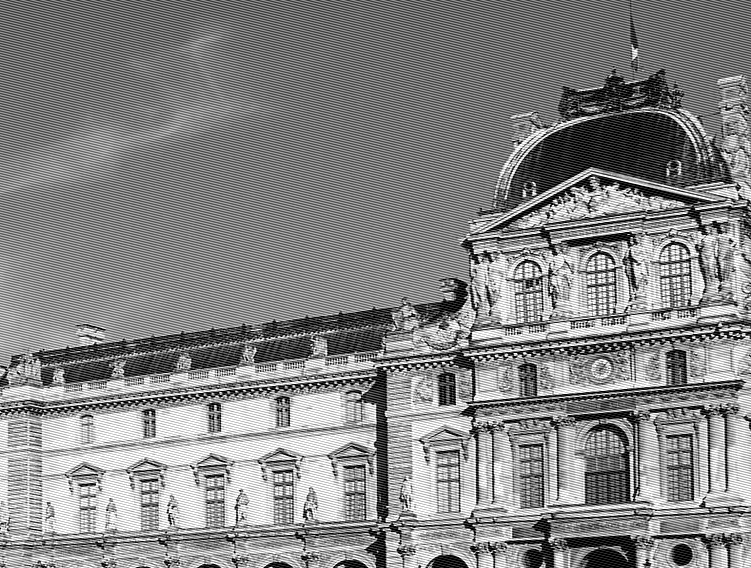
\includegraphics[scale=0.6]{img/monument.png}
			\caption{monument.bmp}
			\label{img1}
		\end{figure}

	\subsection{Représentation fréquentielle de l'image monument.bmp}

		On affiche l'image dans le domaine fréquentiel grâce à une FFT sur deux dimensions.
		
		\begin{figure}[h]
			\centering
			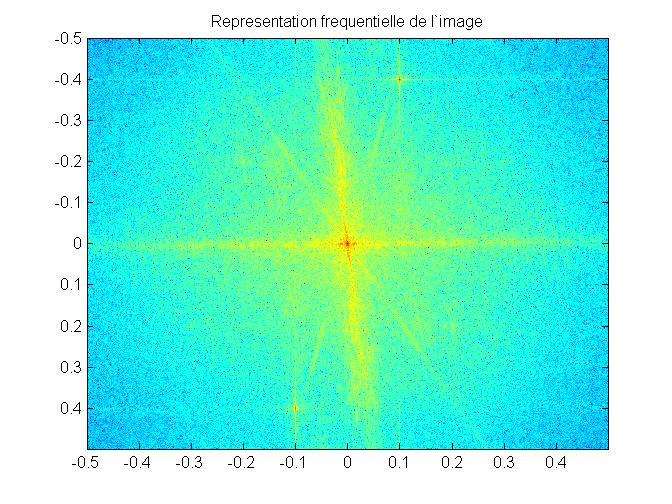
\includegraphics[scale=0.8]{img/img2.png}
			\caption{Représentation fréquentielle}
			\label{img2}
		\end{figure}
		
		On remarque que le bruit se présente sous la forme d'un dirac localisé aux coordonnées $x=0.0992$ et $y=-0.3996$. L'objectif est de le fitrer.

\section{Creation d'un filtre "coupe-bande" de type gaussien}

	\subsection{Creation d'un filtre "passe-bas" de type gaussien}
	
	Dans un premier temps, on génère un filtre "passe-bas" défini par une fonction gaussienne 2D centrée et isotrope dont l'expression est :
	\[ G(x,y) = \frac{1}{2\pi\sigma^2}exp({-\frac{x^2+y^2}{2\sigma^2}}) \]

		\begin{figure}[h]
			\centering
			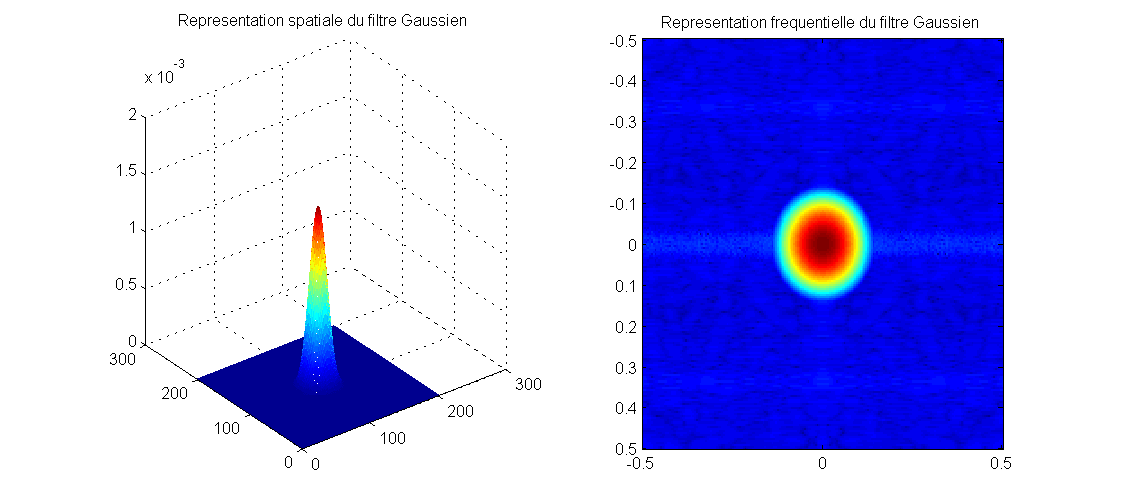
\includegraphics[scale=0.65]{img/img3.png}
			\caption{Représentation spatiale (gauche) et fréquentielle (droite) du filtre}
			\label{img3}
		\end{figure}

	Le filtre a été dimensionné pour obtenir les meilleurs performances lors du filtrage du bruit de l'image monument.bmp. Ainsi, le nombre de points du filtre a été défini à $201*201$ et $\sigma$ à 10.
	
	\subsection{Modulation du filtre "passe-bas" par un signal sinusoïdal}
	
	On module ensuite le filtre précédemment obtenue par un signal sinusoïdal afin de le centrer sur la fréquence parasite et de le transformer en un filtre "passe-bande".
	
		\begin{figure}[H]
			\centering
			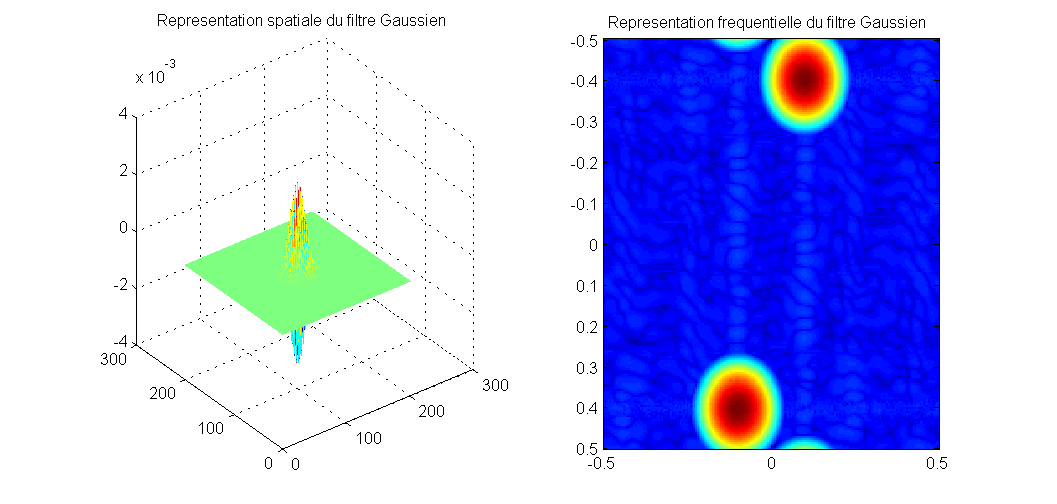
\includegraphics[scale=0.65]{img/img4.png}
			\caption{Représentation spatiale (gauche) et fréquentielle (droite) du filtre}
			\label{img4}
		\end{figure}

\subsection{Tranformation du filtre en un filtre "coupe-bande"}

	Afin d'obtenir un filtre "coupe-bande", permetant de filtrer le bruit de l'image, on crée un dirac dont on soustrait l'expression du filtre précédent. On obtient ainsi un filtre "coupe-bande".

		\begin{figure}[h]
			\centering
			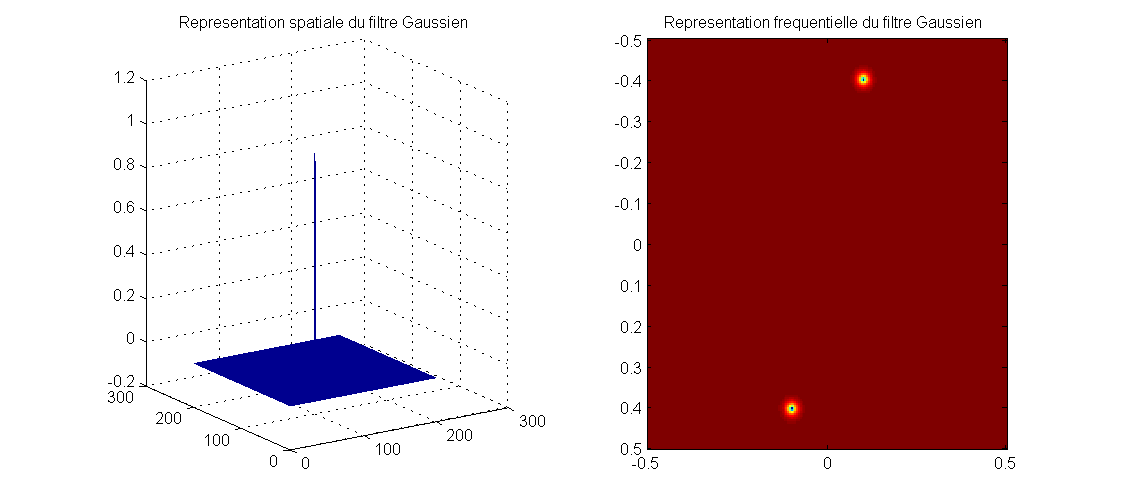
\includegraphics[scale=0.65]{img/img5.png}
			\caption{Représentation spatiale (gauche) et fréquentielle (droite) du filtre}
			\label{img5}
		\end{figure}	

\section{Filtrage de l'image}
	
	\subsection{Représentation de l'image après filtrage}
	
	Après application du filtre précédent, on peut remarquer que le bruit est en très grande partie éliminé. Seuls quelques résidus sont visibles à la périphérie de l'image.
	
	\begin{figure}[H]
			\centering
			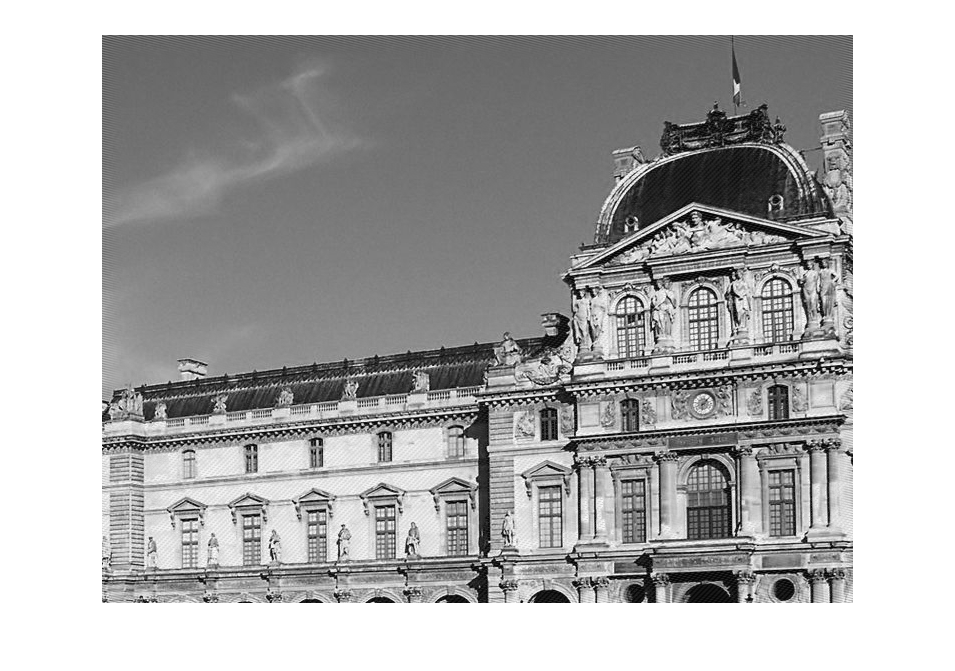
\includegraphics[scale=0.6]{img/monument_filtre.png}
			\caption{Représentation de l'image filtrée}
			\label{monument_filtre}
		\end{figure}


	\subsection{Représentation fréquentielle de l'image après filtrage}
	
	Enfin, en représentant l'image filtrée dans le domaine fréquentiel, on remarque que le dirac n'est presque plus visible, mettant ainsi en évidence l'efficacité du filtre.
	
	\begin{figure}[h]
			\centering
			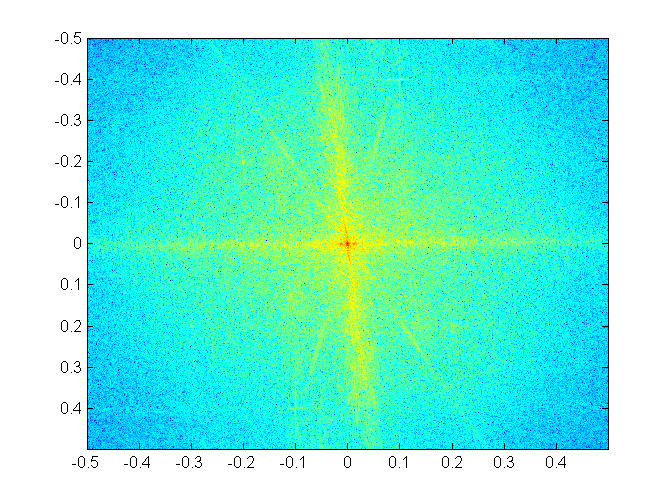
\includegraphics[scale=0.7]{img/img6.png}
			\caption{Représentation fréquentielle de l'image filtrée}
			\label{img6}
		\end{figure}

\end{document}
